


\begin{lucido}[Desired Result]
\begin{center}
	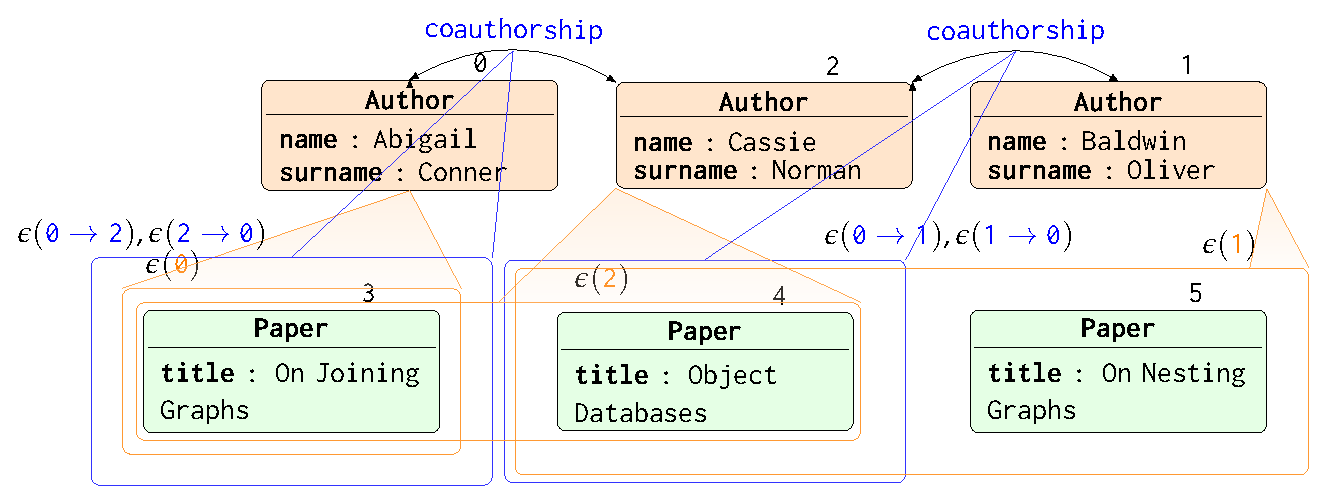
\includegraphics[width=.9\textwidth]{../images/nesting/patterns/042nested.pdf}\\
	Expected result
\end{center}
\end{lucido}

\begin{lucido}[Research Goals]
\begin{enumerate}[<+->]
	\setbeamertemplate{enumerate items}[circle]
	\item As for graph joins, the data model must enhance the \remark{serialization} of both operands and graph result.
	
	\item The logical \remark{graph nesting} operator must be general enough to support both the THoSP algorithm and other graph summarization tasks.
	
	\item Grouping can be avoided by defining a \remark{nesting index}, through which the containment is associated to the container. This can be achieved by extending the Graph Join's data structures with the aforementioned data structure.
	
	%\item The operands' representations model should support property hash joins for backward compatibility.
\end{enumerate}
\end{lucido}
